%% \documentclass[a4paper,twocolumn]{article}
\documentclass[a4paper]{article}

%%%%%%%%%%%%%%%%%%%%%%%%%%%%%%%%%%% PREFERENCES %%%%%%%%%%%%%%%%%%%%%%%%%%%%%%%%%%
% set margin specifics
\usepackage[a4paper, total={6.5in, 9in}]{geometry}

% set unicode
\usepackage[utf8]{inputenc}

% set indent for paragraph
\setlength{\parindent}{2em}

% set graphics support
\usepackage{graphicx}

% setting line spaceing
\renewcommand{\baselinestretch}{2.0}

% use boldface in latex equation
\usepackage{bm}

% Extra math feature
\usepackage{amssymb}
\usepackage{amsmath}

% Code block
\usepackage{listings}
\lstset{
    basicstyle=\footnotesize\ttfamily,
    breaklines=true,
}

% Set the font for lstinline
\makeatletter
\lstdefinestyle{lststyle}{
  basicstyle=%
    \ttfamily
    \color{black}%
    \lst@ifdisplaystyle\scriptsize\fi
}
\makeatother
\lstset{style=lststyle}

% Color
\usepackage{xcolor}

% A better enumerate tool that allows changing the label of item
% It has compatibility issue with beamer;
\usepackage{enumitem}

% Use emojis
\usepackage{pifont}
\usepackage{wasysym}

% No indent
\setlength{\parindent}{0cm}

% Include picture environment
\usepackage[calc]{picture}

% Include TikZ environment
\usepackage{tikz}
\usepackage{calc}

% Include caption
\usepackage{caption}    % !!! For new document
%% \usepackage{caption2}   % !!! Support old document
\usepackage{float}

% Include natbib
\usepackage{natbib}
\setcitestyle{numbers,square}
%% \setcitestyle{authoryear,round}    % Use authoryear format

% Workaround to display bold font in math mode
% Source: https://tex.stackexchange.com/questions/565069/beamer-bold-math-no-longer-working
\DeclareFontShape{OT1}{cmss}{b}{n}{<->ssub * cmss/bx/n}{}

%% \usepackage{setspace}
%% \doublespacing

% To make multirow tables
\usepackage{multirow}

% Use author blocks
\usepackage{authblk}

\newcommand{\PeakNet}{PeakNet}
\newcommand{\peaknet}{PeakNet}
\newcommand{\psocake}{Psocake}
\newcommand{\etal}{\textit{et al}.}
\newcommand{\beSpecific}[1]{(\colorbox{yellow!30}{#1})}
%%%%%%%%%%%%%%%%%%%%%%%%%%%%%%%%%%%%%%%%%%%%%%%%%%%%%%%%%%%%%%%%%%%%%%%%%%%%%%%

% Author block
\renewcommand*{\Authfont}{\normalsize\normalfont}
\renewcommand*{\Affilfont}{\small\itshape}
\author[1]{Cong Wang}
\author[2]{Po-Nan Li}
\author[1]{Jana Thayer}
\author[1,*]{Chun Hong Yoon}
\affil[1]{Linac Coherent Light Source, SLAC National Accelerator Laboratory, Menlo Park, CA, USA.}
\affil[2]{Department of Electrical Engineering, Stanford University, Stanford, CA, USA.}
\affil[*]{Corresponding author: {\textnormal{\texttt{yoon82@slac.stanford.edu}}}}


\begin{document}

% Metadata
% Backward-compatible with latex2e
% Otherwise, it's okay to keep metadata ahead of begin{document}
\title{PeakNet: An Autonomous Bragg Peak Finder with Deep Neural Networks}

\maketitle


\begin{abstract}

Serial crystallography at X-ray free electron laser (XFEL) and synchrotron facilities has experienced tremendous progress in recent times enabling novel scientific investigations into macromolecular structures and molecular processes.  However, these experiments generate a significant amount of data posing computational challenges in data reduction and real-time feedback. Bragg peak finding algorithm is used to identify useful images and also provide real-time feedback about hit-rate and resolution. Shot-to-shot intensity fluctuations and strong background scattering from buffer solution, injection nozzle and other shielding materials make this a time-consuming optimization problem.  Here, we present \peaknet{}, an autonomous Bragg peak finder that utilizes deep neural networks. The development of this system 1) eliminates the need for manual algorithm parameter tuning, 2) reduces false-positive peaks by adjusting to shot-to-shot variations in strong background scattering in real-time, 3) eliminates the laborious task of manually creating bad pixel masks and the need to store these masks per event since these can be regenerated on demand.  \peaknet{} also exhibits exceptional runtime efficiency, processing a $1920 \times 1920$ pixel image around 90 milliseconds for peak finding and mask generation on an NVIDIA 1080 Ti GPU, with the potential for further enhancements through parallelized analysis or GPU stream processing.  \peaknet{} is well-suited for expert-level real-time serial crystallography data analysis at high data rates.

\end{abstract}


\section{Introduction}

Serial crystallography with X-ray free electron lasers (XFEL) has enabled radiation damage-free structural determination of macromolecules at room temperature, an approach commonly known as \textit{diffraction-before-destruction} \citep{neutzePotentialBiomolecularImaging2000, chapmanFemtosecondDiffractiveImaging2006,chapmanFemtosecondXrayProtein2011}.  Time-resolved serial femtosecond crystallography at XFEL facilities, like the Linac Coherent Light Source (LCLS), allows the investigation of biochemical reactions with femtosecond-scale time resolution which has led to many significant structural studies \citep{kupitzSerialTimeresolvedCrystallography2014, nangoThreedimensionalMovieStructural2016,pandeFemtosecondStructuralDynamics2016a, youngStructurePhotosystemII2016,sugaLightinducedStructuralChanges2017, kernStructuresIntermediatesKok2018,ibrahimUntanglingSequenceEvents2020, sugaTimeresolvedStudiesMetalloproteins2020} since the first published work at LCLS \citep{aquilaTimeresolvedProteinNanocrystallography2012}.  In the meantime, the data rate at XFEL facilities have also gradually increased from hundreds of Hz to the MHz range, with the European X-ray Free Electron Laser (EuXFEL) being the first MHz facility available to users and LCLS-II set to launch in 2023.  

At the MHz data rate, novel real-time data analysis approaches are needed to tackle two major challenges that arise in SFX experiments, namely data reduction and real time feedback.  The standard approach for data reduction is vetoing events where the x-ray pulse did not ``hit'' the sample. Typically, hit finding in serial crystallography utilizes Bragg peak finding algorithms implemented in such programs as Cheetah  \citep{bartyCheetahSoftwareHighthroughput2014}, DIALS \citep{winterDIALSImplementationEvaluation2018}, and \psocake{} \citep{yoonPsocakeGUIMaking2020}.  Additionally, a deep neural network-based hit finder for serial crystallography has been reported to achieve a processing rate of 1.3 kHz by analyzing downsized 180 $\times$ 180 images on a single GPU \citep{keConvolutionalNeuralNetworkbased2018}.  Real-time feedback in serial crystallography experiments plays a crucial role by providing users with important information about the experimental conditions.  This enables them to make timely decisions that optimize the data collection process. For instance, it is essential to fine-tune the hit rate to maximize the utilization of samples. Additionally, it is important to monitor factors such as the current diffraction limit, crystalline mosaicity, reciprocal space coverage, and other relevant parameters over time. Therefore, relying solely on hit finding is insufficient to gain the necessary insights, making real-time Bragg peak finding vital for delivering prompt and comprehensive feedback.

In this work, we introduce \peaknet{}, a solution that effectively addresses the challenge of autonomously and efficiently identifying Bragg peaks in high data rate scenarios.  Our approach involves transforming the peak finding problem into a semantic segmentation task, where different regions within diffraction images are classified and segmented using a deep neural network. \peaknet{} autonomously detects Bragg peaks while effectively identifying shot-to-shot variations of strong non-Bragg scattering artifacts, eliminating the need for human intervention.  Subsequently, connected areas of pixels are examined and treated as individual peaks, a task easily accomplished through connected component analysis \citep{weaverCentrosymmetricCrossSymmetricMatrices1985}.  The coordinates of the peaks are determined by calculating the center of mass of all pixels belonging to each identified peak.  Notably, the entire peak finding process is performed on GPUs, offering a cost-effective solution for achieving low latency.


\section{Related work}

Reliable and automatic peak finding algorithms have undergone multiple iterations of development.  An early approach involved utilizing template matching \citep{wilkinsonIntegrationSinglecrystalReflections1988a} based on libraries of peak shapes, but this method was found to be slow and inefficient in runtime, especially when dealing with peaks with low signal-to-noise ratios (SNR).  The main obstacle lies in the localization of peaks and the tuning of user parameters for pattern matching, compounded by the difficult task of developing a comprehensive library of peak shapes.  Another influential approach employed region-growing techniques \citep{bolotovskySeedSkewnessMethodIntegration1995, bartyCheetahSoftwareHighthroughput2014} to detect pixel areas with high skewness.  In the context of serial crystallography with XFEL sources, the efficacy of this method was diminished due to the lack of sufficient data to provide reliable statistics, rendering it susceptible to outliers and less adept in analyzing weak peaks at higher scattering angles, which are essential for achieving atomic resolution in structure determination.

While template matching and region-growing techniques require users to provide prior information like threshold values, Robust Peak Finder (RPF) \citep{hadian-jaziPeakfindingAlgorithmBased2017, hadian-jaziDataReductionSerial2021} has demonstrated proficient peak finding capabilities with minimal user input.  This technique utilizes the Modified Selective Statistical Estimator (MSSE) method to segment background pixels and actual peaks.  Furthermore, the RPF method can also parallelize the processing of diffraction patterns, making it ideal for real-time data analysis.

\psocake{} is a software program specifically designed to streamline high throughput data reduction and analysis of XFEL experiments, and is routinely used at SLAC National Accelerator laboratory (SLAC).  The built-in peak-finding algorithm \citep{shinDataAnalysisUsing2018} includes calibrating raw analog digital units (ADUs); applying optional background correction and bad pixel masks; identifying possible peaks; calculating their SNR; determining Bragg spot sizes; and selecting peaks based on size, total intensity and SNR.

In recent years, neural network models have emerged as a promising avenue for Bragg peak finding.  BraggNet \citep{sullivanBraggNetIntegratingBragg2019} is the first method that demonstrates proficiency of neural network models, specifically U-Net \citep{ronnebergerUNetConvolutionalNetworks2015}, in accurately segmenting peak pixels, including weak peaks, from background pixels in neutron crystallography data.  BraggNet employed simulated peaks to create training datasets, which underwent a number of preprocessing steps, including centering and cropping to a specfic size and adding Poisson noise.  It should be noted that BraggNet works on a single peak at a time within a small 32 by 32 window, which deviates significantly from conventional Bragg peak finding tasks that require extracting peak positions from images typically with hundreds or thousands of pixels along one dimension.  Furthermore, another neural network method for Bragg peak analysis was detailed in the work of BraggNN \citep{liuBraggNNFastXray2021}, emphasizing the refinement of Bragg peak positions without the need for explicit fitting of a profile function, such as the pseudo-Voigt profile.  Likewise, BraggNN works on a single peak at a time within a 11 by 11 window, performing regression to two variables representing the peak position.  To the best of our knowledge, no existing neural network based peak-finding models have demonstrated the ability to detect multiple peaks, which is the primary goal we strive to achieve with \peaknet{}.


\section{Methods}

The current peak finding process of \peaknet{} comprises of two steps, as depicted in Fig. \ref{fig : peak finding}.  First, a segmentation map is obtained from the input image using a deep neural network.  Subsequently, peak positions are determined based on the generated segmentation map using connected component analysis \citep{weaverCentrosymmetricCrossSymmetricMatrices1985}.  Importantly, \peaknet{} has the capability to process inputs with arbitrary image sizes in batches, enabling efficient analysis.

In this section, our focus is to provide a comprehensive description of the underlying deep neural network components in \peaknet{}.  We will specifically discuss the network architecture, data augmentation techniques, and the loss function employed during the training process.  Furthermore, we will emphasize the use of iterative data curation in addressing the outlier problem.

\begin{figure*}[!ht]
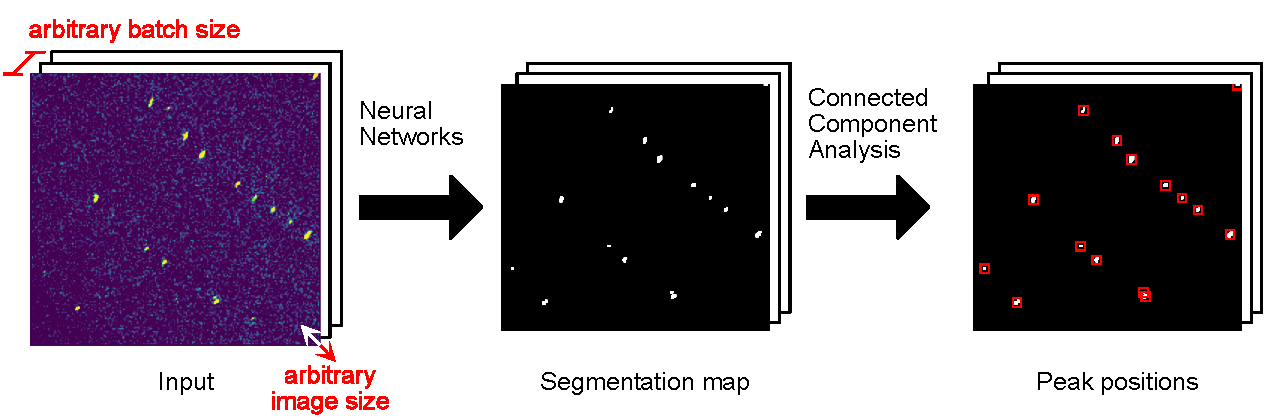
\includegraphics[width=\textwidth,keepaspectratio]
{./figures/peaknet_steps.pdf}
\caption{The peak finding process of \peaknet{} consists of two steps: (1)
obtaining a segmentation map from the input using the underlying deep neural
network; (2) identifying peak positions based on the generated segmentation map
using connected component analysis.  It is worth noting that \peaknet{} is
capable of accommodating input with arbitrary image sizes and batch sizes.  }
\label{fig : peak finding}
\end{figure*}


\subsection{Neural network architecture}

The underlying neural network architecture of \peaknet{} is illustrated in Figure \ref{fig : network arc} (a).  It employs a residual attention U-Net architecture, comprising three main components: a feature extraction ``backbone", a feature fusion ``neck", and a single prediction ``head".  The feature extraction ``backbone" utilizes multiple residual double convolutional blocks to extract multi-resolution features, as visualized in Figure \ref{fig : network arc} (b).  In the feature fusion ``neck", low-resolution features are merged with high-resolution features using gated feature fusion blocks, as depicted in \ref{fig : network arc} (c).  Each block incorporates an attention gate that enhances shared features within both low and high-resolution feature maps.  The resulting combined features from each gated feature fusion block are then rearranged by a subsequent residual double convolutional block.  Finally, to accomplish the segmentation task, the prediction ``head" leverages fused features from the ``neck" and generates a prediction map encompassing three distinct labels: background, Bragg peak, and artifact scattering.  The ``head" itself consists of a 1 $\times$ 1 convolutional layer followed by a softmax function.

Our neural network architecture is primarily based on the original ``Attention U-Net" design \citep{oktayAttentionUNetLearning2018}.  However, we want to point out that the three-component design, consisting of the ``backbone", ``neck" and ``head", offers the flexibility to replace these components with different architectures.  For instance, the ``backbone" can be substituted with a ResNet \citep{heDeepResidualLearning2016}, while the ``neck" can be replaced with other multi-resolution feature fusion methods like feature pyramid networks (FPN) \citep{linFeaturePyramidNetworks2017} or bidirectional feature pyramid networks (BiFPN) \citep{tanEfficientDetScalableEfficient2020}.  Additionally, the ``head" can be extended to perform additional tasks, if desired, such as predicting the likelihood of the input image being indexable.  This modular approach provides flexibility and allows for customization based on specific requirements.

\begin{figure*}[!ht]
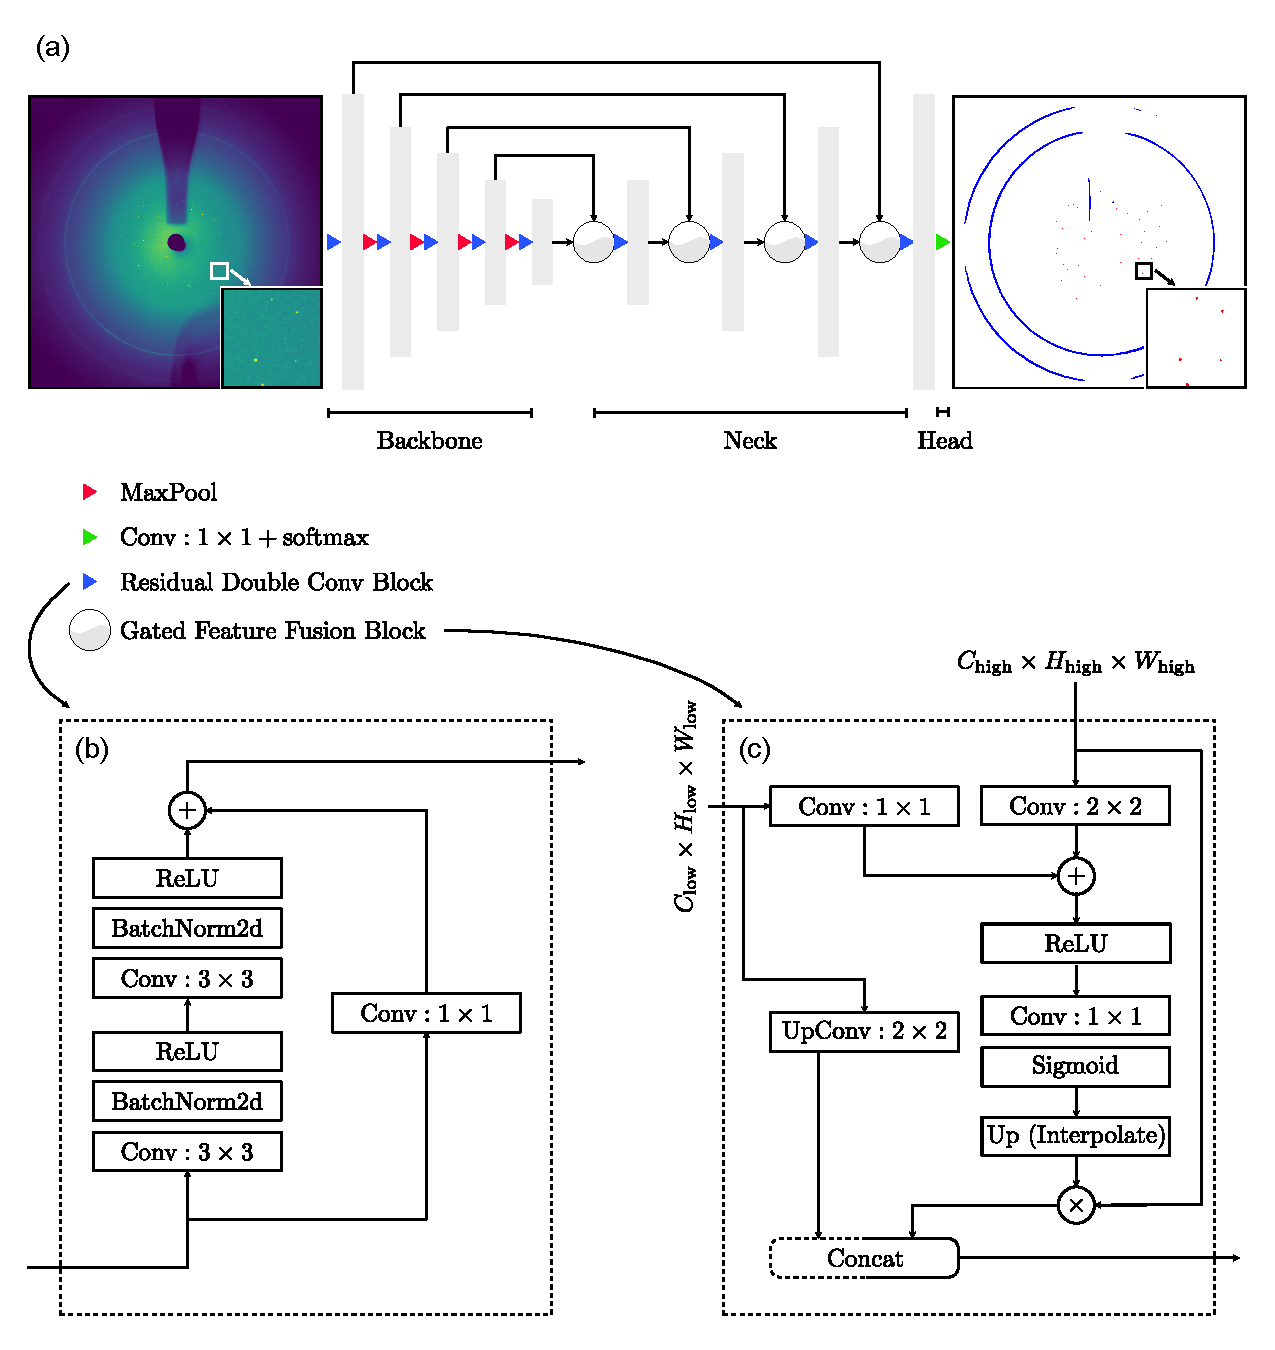
\includegraphics[width=\textwidth,keepaspectratio]
{./figures/network_arc.pdf}
\caption{Neural network architecture: Attention U-Net with residual connections.
(a) Overall end-to-end network architecture.  (b) Residual double
convolutional block.  (c) Gated feature fusion block for merging
multi-resolution features.}
\label{fig : network arc}
\end{figure*}


\subsection{Focal loss as the loss function}

One main technical issue in training neural networks for Bragg peak segmentation is the extreme peak-background class imbalance (e.g., less than $1 : 10^3$), resulting in reduced prediction accuracy.  This may not pose as a problem in previous peak finders like BraggNet, which operates on a much smaller area of $32 \times 32$, \peaknet{} is trained on larger detectors, such as the Rayonix MX340-XFEL detector with a dimension of 1920 $\times$ 1920 pixels even after $4 \times 4$ pixel binning.  To mitigate the label imbalance, we employ a categorical focal loss to address the problem \citep{linFocalLossDense2018}.

\begin{align}
\text{CFL} &= - \sum_{i = 1}^{N}\sum_{j = 1}^{C} 
            \alpha_j \cdot y_j^{(i)} \cdot (1-\hat{p}_j^{(i)})^\gamma 
            \cdot \log{\hat{p}_j^{(i)}}, \\
\hat{p}_j^{(i)} &= f_\theta(x_j^{(i)})
\end{align}

where CFL stands for categorical focal loss, $\alpha_j$ is a balancing factor for each class, $y_j^{(i)}$ is the ground truth label of the $j$-th class for the $i$-th pixel.  $p_j^{(i)}$ is the predicted probability of the $j$-th class for the $i$-th pixel, calculated by the neural network $f$ parameterized by $\theta$ given input image $x_j^{(i)}$ with $N$ number of pixels and $C$ categories.  $\gamma$ is a parameter controlling the extent to which the weight of well-classified examples, such as background pixels, is reduced.  In our neural network training, we chose $\gamma = 2.0$, essentially, this means $(1-\hat{p}_j^{(i)}) ^\gamma$ is solely responsible for down-weighting easy examples, as $\hat{p}_j^{(i)}$ is usually large in this case.  Finding the ideal values for $\alpha$ can be a delicate process with only marginal returns, as highlighted in the original focal loss study \citep{linFocalLossDense2018}.  In order to fully utilize focal loss, we decided to use a fixed trivial value of $\alpha = 1.2$ for all examples, primarily for the sake of completeness.  This choice essentially treats $\alpha$ as a simple scaling factor without significant impact.  In most cases, the sum of all $\alpha_j$ values, denoted as $\sum_{j = 1}^{C} \alpha_j$, sums to 1.


\subsection{Data augmentation}

We applied three data augmentation techniques to each diffraction pattern in our dataset, including random in-plane rotation, random shifting in both horizontal and vertical directions and random masking.  Random in-plane rotation and shifting augment the training data, reducing the model's tendency to memorize features at specific locations.  This variability promotes more generalized feature extraction and improved generalization performance.  Random masking involves randomly obscuring parts of the input data, forcing the model to learn other relevant features that enhance its predictive capabilities during training. 50 rectangular masks with random sizes between 80 and 120 were positioned randomly. The result of applying data augmentation to an arbitrary example is shown in Fig. \ref{fig : data aug}.

\begin{figure*}[!ht]
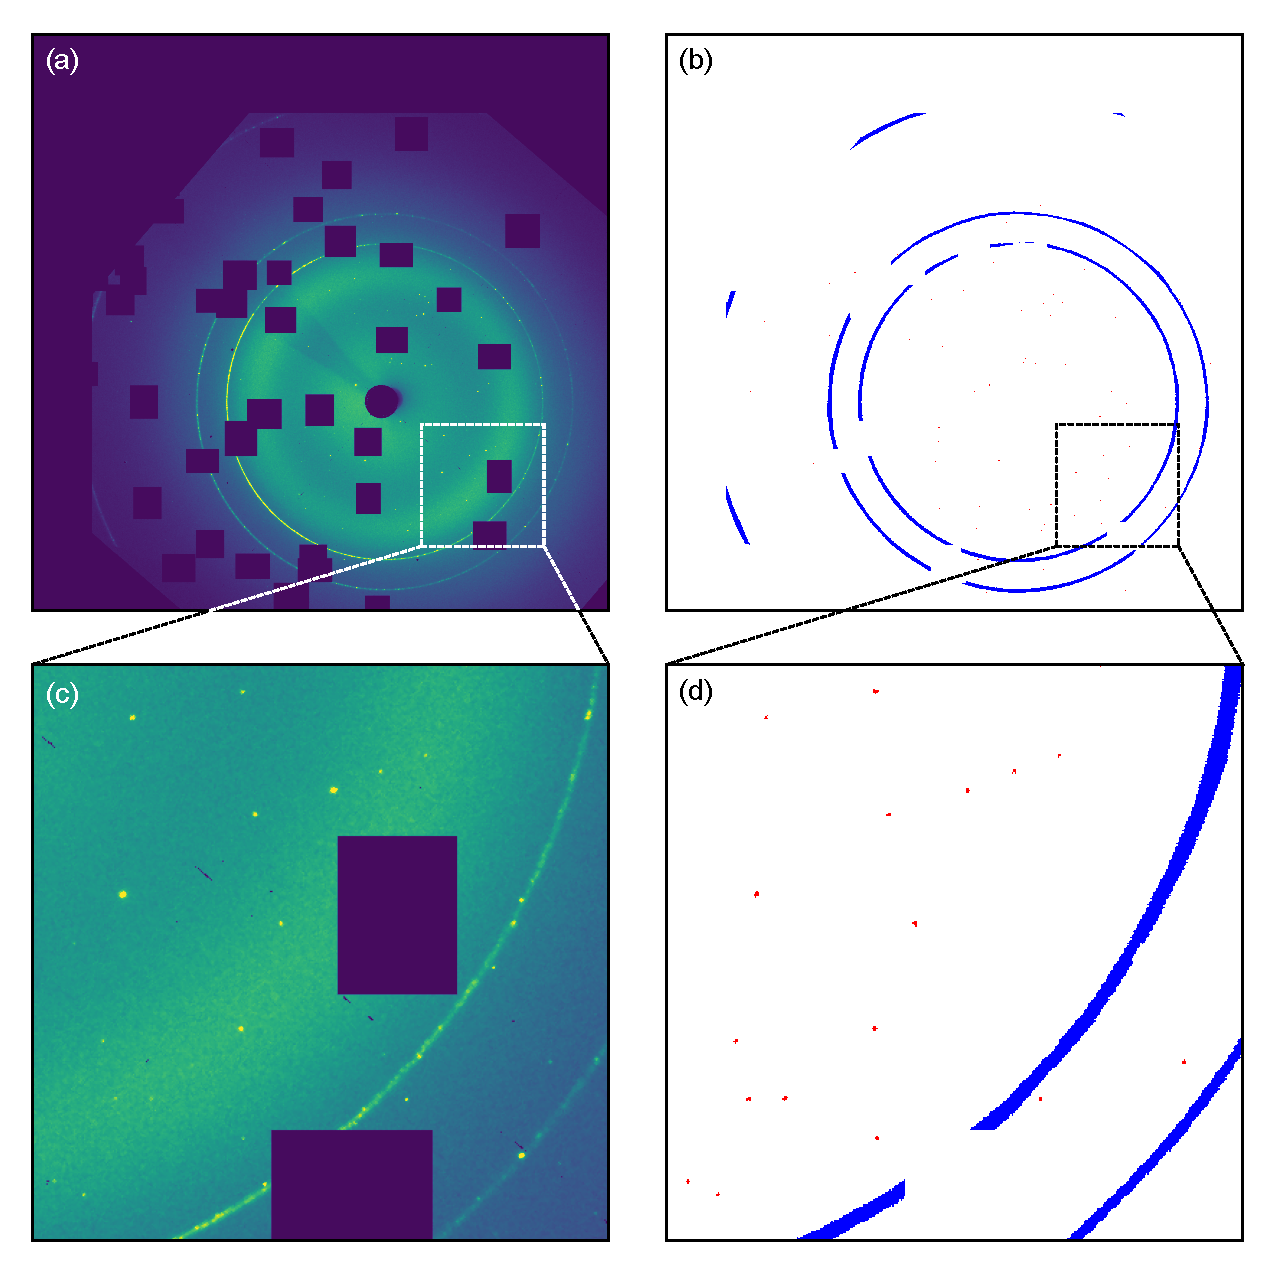
\includegraphics[width=\textwidth,keepaspectratio]
{./figures/data_aug.pdf}
\caption{Illustration of data augmentation on an input image. (a) Augmented
image with random in-plane rotation, shift, and masking. (b) its corresponding
labeled segmentation map. (c, d) Zoomed-in views of (a) and (b), respectively.
The segmentation label distinguishes red pixels as peaks and blue pixels as
artifact scattering, attributed to scattering from metal shielding and injection
nozzle.}
\label{fig : data aug}
\end{figure*}


\subsection{Dataset improvement and correction}

\peaknet{} employs a data-driven approach to accurately identify Bragg peaks, requiring dataset improvement and correction to enhance performance.  This contrasts with model-driven approaches that primarily entail direct model modification to improve capabilities.  Fig. \ref{fig : data engine} illustrates a feedback loop for iterative dataset improvement and correction.  

The process begins with the preparation of a source dataset, often accomplished through a combination of algorithmic and manual data labeling.  Subsequently, the deep neural networks within \peaknet{} are trained on this dataset to learn how to accurately detect peaks.  Following training, the model is deployed to predict peaks on previously unseen data, and its performance is thoroughly evaluated.  During this evaluation, instances that notably worsen the performance of \peaknet{} are identified.  To address these limitations, we either correct low-quality labels predicted by the neural networks or, alternatively, acquire additional data that closely resemble these challenging instances and carefully annotate them.  Finally, we merge these newly labeled instances into the training set and retrain the model, thereby improving its overall performance.  

Interestingly, during the initial pass of this iterative process, \peaknet{} showed limited performance when dealing with images containing relatively low levels of photons.  However, by obtaining and annotating these images, we were able to enhance the training dataset and, as a result, significantly improve the predictive performance of \peaknet{}.


\begin{figure}[!ht]
\centering
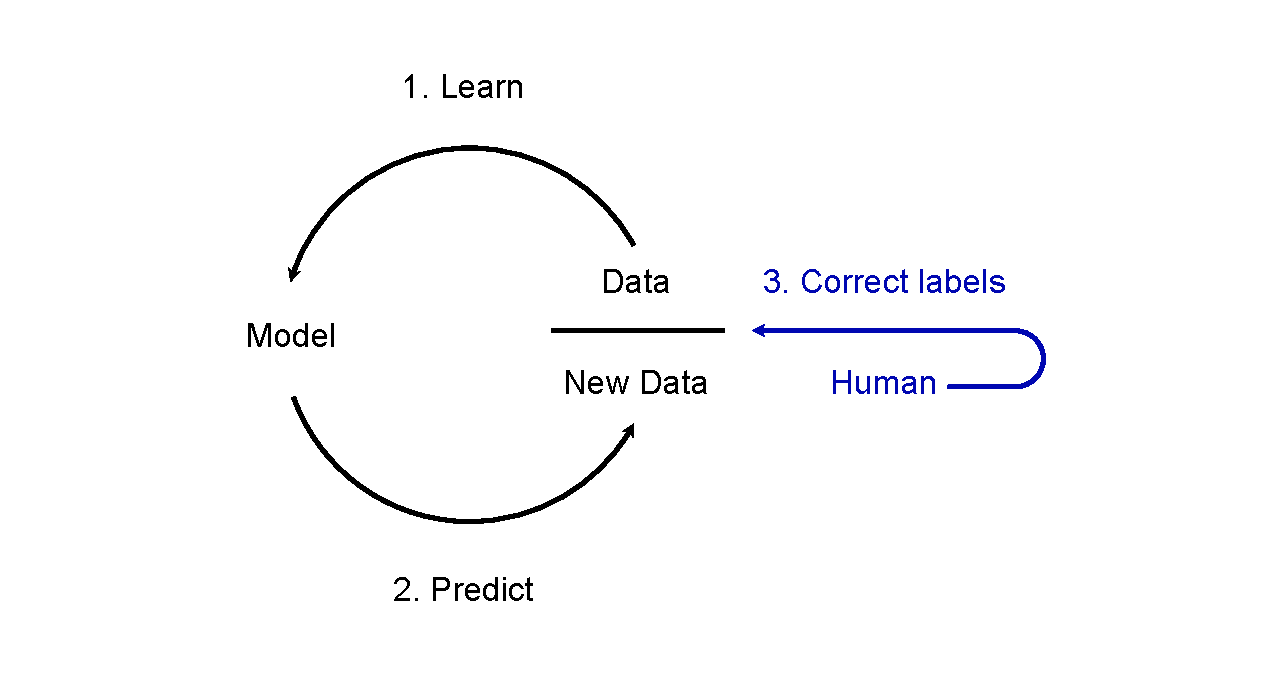
\includegraphics[width=\columnwidth,keepaspectratio,trim={1in 0in 1in 0in}]
{./figures/data_engine.pdf}
\caption{The three step process of iterative dataset and model improvement. (1) Model learns from training data. (2) Model predictions reveal potential areas of improvement. (3) Correct low-quality training labels or acquire additional examples of challenging instances.}
\label{fig : data engine}
\end{figure}


\section{Results}

The primary goal of \peaknet{} is to autonomously detect Bragg peaks in diffraction images, devoid of any user input, such as algorithmic parameter tuning or manual artifact masking.  We implemented a two-step approach for peak detection, employing deep neural networks to perform semantic segmentation, which was subsequently followed by connected component analysis to extract image coordinates of Bragg peaks.  In this section, we begin by introducing the datasets used for training, validating, and testing \peaknet{}. Next, we present the evaluation results that demonstrate the predictive performance of \peaknet{}. Finally, we showcase its auto-masking capability and runtime efficiency.


\subsection{Dataset}

We obtained X-ray diffraction images from two experiments conducted at the Macromolecular Femtosecond Crystallography (MFX) instrument within LCLS.  The primary dataset utilized for training and evaluating \peaknet{} is ``mfx13016" (Run number: 28,31-34, 36-38), which contains diverse biological samples, e.g.  thaumatin and proteinase, and this experiment was originally used for automated drop dispensing research \citep{suSerialCrystallographyUsing2021}.  These diffraction images were recorded on a Rayonix MX340-XFEL detector with a dimension of 1920 $\times$ 1920, downsized by a factor of 4 to accommodate a higher readout rate.  

The dataset ``mfx13016" exhibits a notable ring-like background scattering accompanied by bright Bragg peak-like spots located on the rings.  This characteristic presents two primary challenges for crystallography data analysis: increased difficulty in crystal indexing due to false-positive peaks and inaccurate integration results caused by artifact scattering.  The current best practice involves manual masking of these artifact scattering, enabling data analysis to proceed as if they are absent, but this process is time-consuming and can not adjust to shot-to-shot variations in the artifacts in real-time.  Additionally, the final outcomes often hinge on the expertise of the individuals conducting the data processing, resulting in biases, scalability limitations, lack of standardization, and the possibility of human errors.  Nevertheless, the inherent challenges presented by this dataset offer an exceptional opportunity to showcase the autonomous peak finding capability of \peaknet{}.

The neural network training dataset consists of 98 Rayonix images in run 28 of ``mfx13016", which includes thaumatin samples, and an additional 37 images sampled from an internal LCLS experimental dataset related to therapeutics development associated with SARS-CoV-2.  Incorporating the SARS-CoV-2 dataset aims to educate \peaknet{} about the presence of images without artifact rings, diversifying its understanding of different data characteristics.  Nonetheless, all these images used for neural network training have a dimension of 1920 $\times$ 1920 and they are divided into an 80\% training set and a 20\% validation set.  The final test dataset for evaluating the model comprises all images in run 31-34 and run 36-38 of ``mfx13016".


\subsection{Evaluating \peaknet{}'s predictive performance}

The peak finding performance of peak finders is evaluated through three key indicators from a user's standpoint: the number of successfully indexed hits, the indexing rate, and the merging statistics.  For our evaluation, we utilized the CrystFEL software suite \citep{whiteCrystFELSoftwareSuite2012} to perform crystal indexing, integration, and merging tasks.  We use \psocake{}'s peak finder as a baseline in this evaluation.

\subsubsection{Indexing results}

\peaknet{} and manually fine-tuned \psocake{} exhibit comparable peak finding performance in terms of the number of hits and the number of indexed images, as shown in Table \ref{tb : index}.  However, we emphasize that while \peaknet{} operates entirely autonomously, \psocake{}'s performance is contingent upon manual parameter fine-tuning and manual artifact scattering masking.  For example, an earlier work \citep{suSerialCrystallographyUsing2021}, which processed the same experimental data, reported significantly lower hit count and indexed image count.  Consequently, this highlights \peaknet{}'s advantage in user-independent expert-level data processing.

Moreover, while users might prioritize the absolute number of indexed images as a more straightforward metric, the indexing rate provides valuable insights into the method's efficiency.  Both metrics jointly offer a more comprehensive evaluation of the peak finding method. In the case of \peaknet{}, both consistently high number of indexed images and high indexing rate testify to its effective and reliable autonomous peak finding process.


\begin{table*}

\caption{Comparison of crystal indexing results for different methods on the
test dataset.  The table shows the number of hits, number of indexed hits, and
indexing rates for \peaknet{}, \psocake{} (fine-tuned) and \psocake{} (Su 2021).
The ``Run (Samples)" column lists the specific run numbers and biological
samples (TH: thaumatin; PK: proteinase).}

\label{tb : index}

\resizebox{1.0\textwidth}{!}{
\begin{tabular}{lllllllll}
\hline
\multicolumn{1}{l}{Methods}                                                                            & \multicolumn{1}{l}{Run (Samples)}        & \multicolumn{1}{l}{31 (TH)} & \multicolumn{1}{l}{32 (TH)} & \multicolumn{1}{l}{33 (TH)} & \multicolumn{1}{l}{34 (TH)} & \multicolumn{1}{l}{36 (TH)} & \multicolumn{1}{l}{37 (PK)} & 38 (PK) \\ \hline
\multicolumn{1}{l}{\multirow{3}{*}{\peaknet{}}}                                                        & \multicolumn{1}{l}{Number of hits}       & \multicolumn{1}{l}{\textbf{1205}}    & \multicolumn{1}{l}{\textbf{3248}}    & \multicolumn{1}{l}{\textbf{5797}}    & \multicolumn{1}{l}{\textbf{3949}}    & \multicolumn{1}{l}{\textbf{1184}}    & \multicolumn{1}{l}{1030}    & \textbf{1223}    \\ \cline{2-9}
\multicolumn{1}{l}{}                                                                                   & \multicolumn{1}{l}{Number of indexed}    & \multicolumn{1}{l}{\textbf{860}}     & \multicolumn{1}{l}{\textbf{2856}}    & \multicolumn{1}{l}{\textbf{3433}}    & \multicolumn{1}{l}{\textbf{2401}}    & \multicolumn{1}{l}{\textbf{919}}     & \multicolumn{1}{l}{953}     & 1169    \\ \cline{2-9}
\multicolumn{1}{l}{}                                                                                   & \multicolumn{1}{l}{Indexing rate}        & \multicolumn{1}{l}{\textbf{0.71}}    & \multicolumn{1}{l}{\textbf{0.88}}    & \multicolumn{1}{l}{\textbf{0.59}}    & \multicolumn{1}{l}{\textbf{0.61}}    & \multicolumn{1}{l}{0.78}    & \multicolumn{1}{l}{0.93}    & 0.96    \\ \hline
\multicolumn{9}{l}{}                                                                                                                                                                                                                                                                                                                                \\ \hline
\multicolumn{1}{l}{\multirow{3}{*}{\begin{tabular}[c]{@{}l@{}}\psocake{}\\ (fine-tuned)\end{tabular}}} & \multicolumn{1}{l}{Number of hits}       & \multicolumn{1}{l}{1193}    & \multicolumn{1}{l}{3087}    & \multicolumn{1}{l}{5769}    & \multicolumn{1}{l}{3926}    & \multicolumn{1}{l}{917}     & \multicolumn{1}{l}{\textbf{1070}}    & 1212    \\ \cline{2-9}
\multicolumn{1}{l}{}                                                                                   & \multicolumn{1}{l}{Number of indexed}    & \multicolumn{1}{l}{849}     & \multicolumn{1}{l}{2657}    & \multicolumn{1}{l}{3375}    & \multicolumn{1}{l}{2364}    & \multicolumn{1}{l}{760}     & \multicolumn{1}{l}{\textbf{1005}}    & \textbf{1202}    \\ \cline{2-9}
\multicolumn{1}{l}{}                                                                                   & \multicolumn{1}{l}{Indexing rate}        & \multicolumn{1}{l}{\textbf{0.71}}    & \multicolumn{1}{l}{0.86}    & \multicolumn{1}{l}{\textbf{0.59}}    & \multicolumn{1}{l}{0.60}     & \multicolumn{1}{l}{\textbf{0.83}}    & \multicolumn{1}{l}{\textbf{0.94}}    & \textbf{0.99}    \\ \hline
\multicolumn{9}{l}{}                                                                                                                                                                                                                                                                                                                                \\ \hline
\multicolumn{1}{l}{\multirow{3}{*}{\begin{tabular}[c]{@{}l@{}}\psocake{}\\ (Su2021) \end{tabular}}}    & \multicolumn{1}{l}{Number of hits}       & \multicolumn{1}{l}{1083}    & \multicolumn{1}{l}{2454}    & \multicolumn{1}{l}{5604}    & \multicolumn{1}{l}{3756}    & \multicolumn{1}{l}{363}     & \multicolumn{1}{l}{683}     & 771     \\ \cline{2-9}
\multicolumn{1}{l}{}                                                                                   & \multicolumn{1}{l}{Number of indexed}    & \multicolumn{1}{l}{271}     & \multicolumn{1}{l}{1094}    & \multicolumn{1}{l}{963}     & \multicolumn{1}{l}{770}     & \multicolumn{1}{l}{266}     & \multicolumn{1}{l}{569}     & 709     \\ \cline{2-9}
\multicolumn{1}{l}{}                                                                                   & \multicolumn{1}{l}{Indexing rate}        & \multicolumn{1}{l}{0.25}    & \multicolumn{1}{l}{0.45}    & \multicolumn{1}{l}{0.17}    & \multicolumn{1}{l}{0.21}    & \multicolumn{1}{l}{0.73}    & \multicolumn{1}{l}{0.83}    & 0.92    \\ \hline
\end{tabular}
}

\end{table*}


\subsubsection{Merging statistics}

Merging statistics confirms \peaknet{}'s robust performance in terms of consistency and quality in data processing.  For the thaumatin (TH) sample, \peaknet{} demonstrates marginally superior performance in terms of R-split values, correlation coefficients, $I/\sigma(I)$ values, redundancy, and completeness, achieving these results autonomously.  Notably, the R-split value for thaumatin is slightly lower for \peaknet{} (0.2605 vs. 0.2732), suggesting slightly better internal consistency. Similarly, correlation coefficients for \peaknet{} are marginally higher (CC$_1/2$: 0.9434 vs.  0.9368; CC*: 0.9853 vs. 0.9835), indicating a minor advantage in the precision of measurements.

However, for the proteinase (PK) sample, the performance comparison is mixed.  Although \peaknet{} lags slightly behind manually fine-tuned \psocake{} in terms of R-split and redundancy, it outperforms in CC$_1/2$, CC*, $I/\sigma(I)$, and completeness values.  This reinforces the effectiveness of \peaknet{} in achieving respectable results across varied sample types, without any manual intervention or parameter fine-tuning.  

Overall, \peaknet{} demonstrates comparable performance to a manually fine-tuned \psocake{} for two distinct samples, showcasing its potential for autonomous peak finding with consistent results.  By reducing dependence on the expertise of individuals, which can have considerable variation, \peaknet{} offers a promising user-independent solution.  Notably, despite primarily being trained on PK samples, \peaknet{} maintains robust and versatile performance, indicating its broad applicability and effectiveness in handling diverse datasets.


\begin{table*}
\caption{Comparison of merging statistics between \peaknet{} and fine-tuned \psocake{}.  Thaumatin (TH) results were
merged from run 31, 32, 33, 34 and 36. Proteinase (PK) results were merged from run
37 and 38.}
\label{tb : merge}
\centering
\resizebox{1.0\textwidth}{!}{
\begin{tabular}{lllllllll}
\hline
Sample              & Methods & R-split & CC$_{1/2}$     & CC*       & $I/\sigma(I)$   & Resolution range (Å) & Redundancy & Completeness \\ \hline
\multirow{2}{*}{TH} & \peaknet{} & \textbf{0.2605}  & \textbf{0.9434} & \textbf{0.9853} & \textbf{2.0590} & 1.45-27.93           & \textbf{76.05}      & \textbf{0.9594}       \\ \cline{2-9} 
                    & \psocake{} & 0.2732  & 0.9368 & 0.9835 & 2.0277 & \textbf{1.01-31.32}           & 72.20      & 0.9367       \\ \hline
                    &         &         &           &           &          &                      &            &              \\ \hline
Sample              & Methods & R-split & CC$_{1/2}$     & CC*       & $I/\sigma(I)$   & Resolution range (Å) & Redundancy & Completeness \\ \hline
\multirow{2}{*}{PK} & \peaknet{} & 0.7711  & \textbf{0.2234}    & \textbf{0.6043}    & \textbf{1.135}    & 1.45-26.98           & 16.36      & \textbf{0.8668}       \\ \cline{2-9} 
                    & \psocake{} & \textbf{0.7589}  & 0.1900    & 0.5650    & 0.974    & \textbf{1.45-30.04}           & \textbf{17.83}      & 0.8365       \\ \hline
\end{tabular}
}
\end{table*}


\subsection{Auto-masking: predicting scattering artifacts}

Auto-masking functionality in \peaknet{} represents a significant advancement in the automated processing of diffraction images.  The underlying neural network architecture enables \peaknet{} to autonomously discern and segregate pixel regions affected by scattering artifacts, such as distinct ring-like structures produced by metal shielding used to reduce air scatter and/or liquid jet nozzle scattering.  This capability circumvents the need for manual masking in the peak finding process and the need to store a binary mask used for each event which is needed for crystal indexing/integration, thereby optimizing the efficiency of crystallographic data processing.

Fig. \ref{fig : automask 1} provides a comparative visualization of \peaknet{}'s effectiveness in accurately segmenting regions with bright pixels induced by scattering artifacts under various conditions.  Images without ring artifacts are also included in the visualization, reassuring that \peaknet{} does not generate or ``hallucinate" ring artifacts where they do not exist.  This visual representation serves as tangible evidence of \peaknet{} 's adeptness in discriminating and processing pertinent features, regardless of the contextual complexities.

Furthermore, while evaluating \peaknet{}'s auto-masking feature on intended input images, we explored its behavior on unintended inputs, providing insights into its robustness and generalizability.  Fig. \ref{fig : automask 2} depicts illustrative examples of \peaknet{} predicting artifact scattering patterns in silver behenate scattering captured on various detectors. Silver behenate is a popular calibrant used to determine the detector position relative to the beam based on the known ring spacing. Surprisingly, \peaknet{} reliably identifies the characteristic scattering ring structures present in silver behenate images.  This observation provides compelling evidence once again, further demonstrating the robust predictive capability of \peaknet{} in accurately recognizing artifact scattering patterns.  As a result, it reinforces that effectiveness of \peaknet{}'s auto-masking feature and the potential to automatically optimize the diffraction geometry.


\begin{figure*}[!ht]
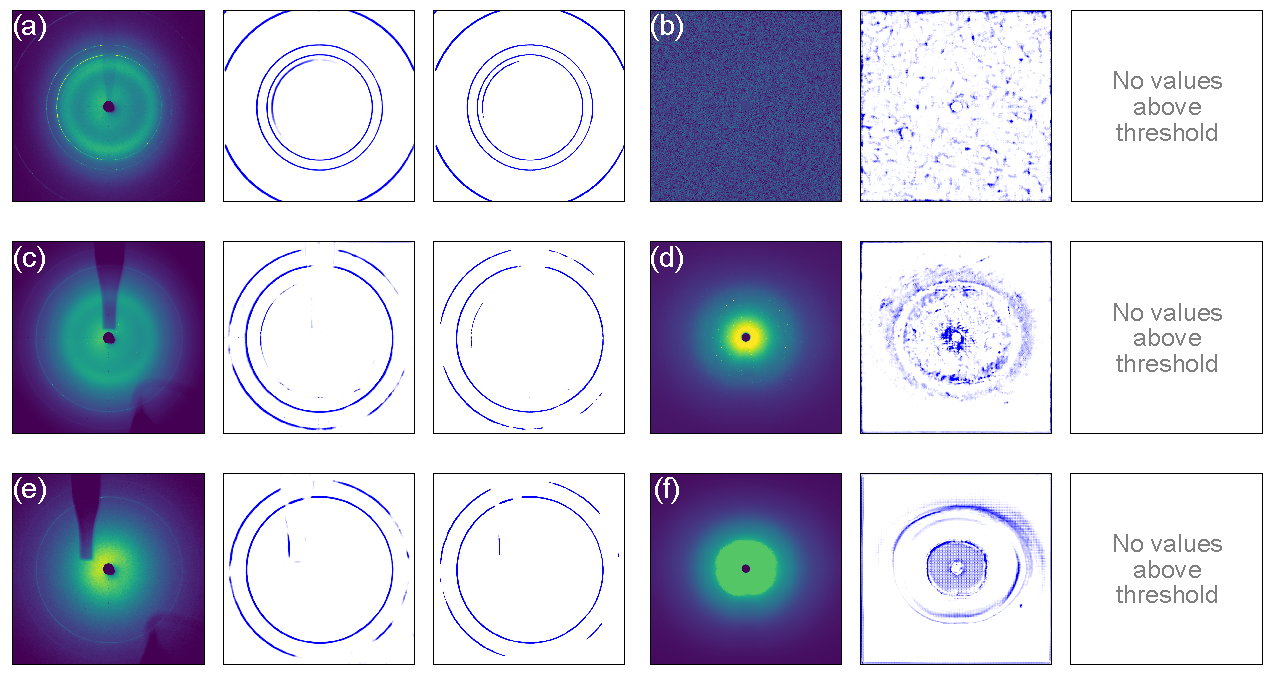
\includegraphics[width=\textwidth,keepaspectratio]
{./figures/automask.pdf} 
\caption{Examples of auto-masking using \peaknet{}.  Each panel contains three
images: the original image, the segmentation map used for masking, and the
resulting mask after thresholding.  Panels (a), (c) and (e) show three different
scenarios with artifact scattering rings.  Panels (b), (d) and (f) visualize the
response of \peaknet{} on images without any artifact scattering rings.}
\label{fig : automask 1} 
\end{figure*}


\begin{figure*}[!ht]
\centering
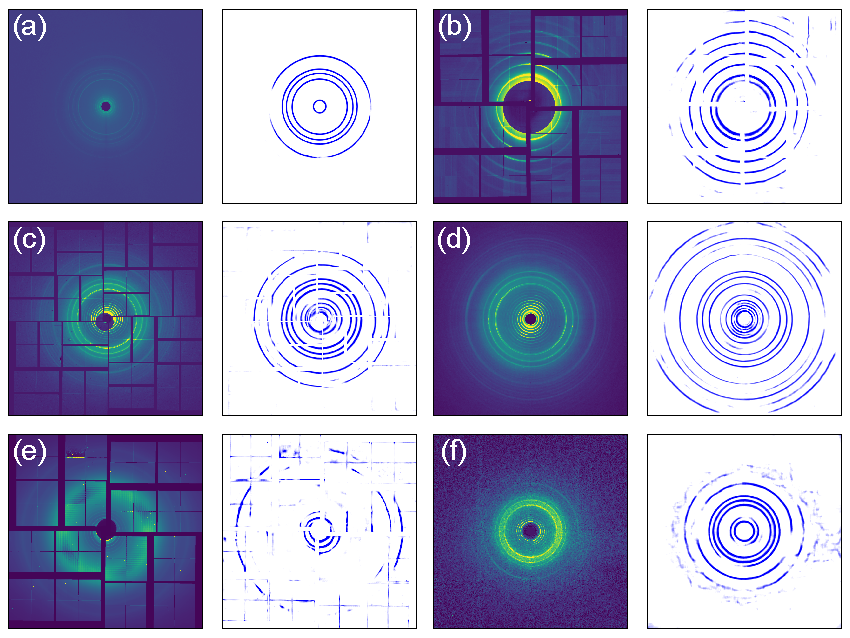
\includegraphics[width=\textwidth,keepaspectratio]
{./figures/automask.agbehnate.pdf}
\caption{Examples of identifying scattering rings in silver behenate images using
\peaknet{}.}
\label{fig : automask 2}
\end{figure*}


\subsection{Runtime efficiency}

Peak finding can pose a significant computational demand, particularly in high data rate experiments, highlighting the critical importance of an efficient peak finding algorithm.  A comparative analysis of runtime performance demonstrates the greater efficiency of \peaknet{} compared to other commonly used \psocake{} peak finder.

When processing Rayonix images with $1920 \times 1920$ pixels, \peaknet{} achieved a significantly reduced processing time of 90 milliseconds per event on an NVIDIA 1080 Ti GPU for peak finding and auto-mask generation.  In contrast, \psocake{} required 176 milliseconds per event when executed on an Intel E5-2620 CPU.  To provide a reference, an earlier study \citep{hadian-jaziDataReductionSerial2021} also reported the runtime efficiency of both the Robust Peak Finder (RBF) and Cheetah, demonstrating an average processing time of around 120 milliseconds for 3 times smaller AGIPD 1M \citep{allahgholiAdaptiveGainIntegrating2019} images.  It should be noted that computation time would be even longer if the auto-masking feature is introduced to these existing peak finders. This result clearly demonstrates that \peaknet{} not only delivers robust Bragg peak finding results autonomously but also exhibits remarkable runtime efficiency.

\begin{table*}[t]
\caption{
    The runtime performance of diffraction image analysis algorithms measured on Rayonix images containing 3.7 megapixels.  We measured runtime performance of \psocake{} and \peaknet{} directly using Rayonix images.  For reference purposes, we also included peak finding methods RPF and Cheetah, whose runtime performance were originally measured on AGIPD 1M.
}
\label{tb : runtime}
\centering
\resizebox{!}{!}{
\begin{tabular}{lllcc}
\hline
Methods         &  Auto-mask   & Hardware       & Image dimension    & Time (ms/event) \\ \hline
\peaknet{}      &  Yes         & NVIDIA 1080 Ti & 1920 $\times$ 1920 & 90.0            \\ \hline
\psocake{}      &  No          & Intel E5-2620  & 1920 $\times$ 1920 & 175.5           \\ \hline
RPF             &  No          & Intel E5-2698  & 1024 $\times$ 1024 & 120.0           \\ \hline
Cheetah         &  No          & Intel E5-2698  & 1024 $\times$ 1024 & 120.0           \\ \hline
%CNN hit finder      & Hit Finding  & NVIDIA 1080 Ti & 720 $\times$ 720   & 0.8             \\ \hline
%ORB+MLP             & Hit Finding  & Intel Core i5  & 720 $\times$ 720   & 50.0            \\ \hline
\end{tabular}
}
\end{table*}


\section{Conclusions}

\peaknet{} exhibits exceptional capabilities in autonomous Bragg peaks finding without requiring user input or intervention, such as algorithmic parameter tuning or manual artifact masking.  The predictive performance of \peaknet{} in peak finding proves to be comparable to, if not better than, manually fine-tuned \psocake{} with user-supplied masks.  An integral feature of \peaknet{}, auto-masking, significantly enhances its ability to autonomously identify and process artifact scattering patterns.  Moreover, the efficiency of \peaknet{} is exemplified by its impressive runtime performance, surpassing commonly used peak finders like \psocake{} and RPF.  Parallel processing with GPU streaming can potentially improve the runtime efficiency even further.  In conclusion, \peaknet{}  offers a robust, versatile, and efficient solution that operates independently of user input, thereby holding significant potential for optimizing crystallographic data processing at high data rates.


\section*{Acknowledgment}

Earlier versions utilizing YOLO and U-Net models were built and tested by P.L and C.H.Y.  The experiments were designed by C.W with inputs from J.B.T and C.H.Y.  C.W implemented the residual attention U-Net, prepared the datasets, labeled experimental data, and trained and evaluated the refined neural network model.  The manuscript was written by C.W and C.H.Y with input from all authors.  This material is based upon work supported by the U.S.  Department of Energy, Office of Science, Office of Basic Energy Sciences under Award Number FWP-100643.  Use of the Linac Coherent Light Source (LCLS), SLAC National Accelerator Laboratory, is supported by the U.S.  Department of Energy, Office of Science, Office of Basic Energy Sciences under Contract No.DE-AC02-76SF00515.  C.W acknowledges the assistance provided by ChatGPT from OpenAI in refining the language and enhancing the readability of this paper.


\begin{thebibliography}{33}
\providecommand{\natexlab}[1]{#1}
\providecommand{\url}[1]{\texttt{#1}}
\expandafter\ifx\csname urlstyle\endcsname\relax
  \providecommand{\doi}[1]{doi: #1}\else
  \providecommand{\doi}{doi: \begingroup \urlstyle{rm}\Url}\fi

\bibitem[Allahgholi et~al.(2019)Allahgholi, Becker, Delfs, Dinapoli,
  Goettlicher, Greiffenberg, Henrich, Hirsemann, Kuhn, Klanner, Klyuev,
  Krueger, Lange, Laurus, Marras, Mezza, Mozzanica, Niemann, Poehlsen,
  Schwandt, Sheviakov, Shi, Smoljanin, Steffen, {Sztuk-Dambietz}, Trunk, Xia,
  Zeribi, Zhang, Zimmer, Schmitt, and
  Graafsma]{allahgholiAdaptiveGainIntegrating2019}
Aschkan Allahgholi, Julian Becker, Annette Delfs, Roberto Dinapoli, Peter
  Goettlicher, Dominic Greiffenberg, Beat Henrich, Helmut Hirsemann, Manuela
  Kuhn, Robert Klanner, Alexander Klyuev, Hans Krueger, Sabine Lange, Torsten
  Laurus, Alessandro Marras, Davide Mezza, Aldo Mozzanica, Magdalena Niemann,
  Jennifer Poehlsen, Joern Schwandt, Igor Sheviakov, Xintian Shi, Sergej
  Smoljanin, Lothar Steffen, Jolanta {Sztuk-Dambietz}, Ulrich Trunk, Qingqing
  Xia, Mourad Zeribi, Jiaguo Zhang, Manfred Zimmer, Bernd Schmitt, and Heinz
  Graafsma.
\newblock The {{Adaptive Gain Integrating Pixel Detector}} at the {{European
  XFEL}}.
\newblock \emph{Journal of Synchrotron Radiation}, 26\penalty0 (1):\penalty0
  74--82, January 2019.
\newblock ISSN 1600-5775.
\newblock \doi{10.1107/S1600577518016077}.

\bibitem[Aquila et~al.(2012)Aquila, Hunter, Doak, Kirian, Fromme, White,
  Andreasson, Arnlund, Bajt, Barends, Barthelmess, Bogan, Bostedt, Bottin,
  Bozek, Caleman, Coppola, Davidsson, DePonte, Elser, Epp, Erk, Fleckenstein,
  Foucar, Frank, Fromme, Graafsma, Grotjohann, Gumprecht, Hajdu, Hampton,
  Hartmann, Hartmann, {Hau-Riege}, Hauser, Hirsemann, Holl, Holton, H{\"o}mke,
  Johansson, Kimmel, Kassemeyer, Krasniqi, K{\"u}hnel, Liang, Lomb, Malmerberg,
  Marchesini, Martin, Maia, Messerschmidt, Nass, Reich, Neutze, Rolles, Rudek,
  Rudenko, Schlichting, Schmidt, Schmidt, Schulz, Seibert, Shoeman, Sierra,
  Soltau, Starodub, Stellato, Stern, Str{\"u}der, Timneanu, Ullrich, Wang,
  Williams, Weidenspointner, Weierstall, Wunderer, Barty, Spence, and
  Chapman]{aquilaTimeresolvedProteinNanocrystallography2012}
Andrew Aquila, Mark~S. Hunter, R.~Bruce Doak, Richard~A. Kirian, Petra Fromme,
  Thomas~A. White, Jakob Andreasson, David Arnlund, Sa{\v s}a Bajt, Thomas
  R.~M. Barends, Miriam Barthelmess, Michael~J. Bogan, Christoph Bostedt,
  Herv{\'e} Bottin, John~D. Bozek, Carl Caleman, Nicola Coppola, Jan Davidsson,
  Daniel~P. DePonte, Veit Elser, Sascha~W. Epp, Benjamin Erk, Holger
  Fleckenstein, Lutz Foucar, Matthias Frank, Raimund Fromme, Heinz Graafsma,
  Ingo Grotjohann, Lars Gumprecht, Janos Hajdu, Christina~Y. Hampton, Andreas
  Hartmann, Robert Hartmann, Stefan {Hau-Riege}, G{\"u}nter Hauser, Helmut
  Hirsemann, Peter Holl, James~M. Holton, Andr{\'e} H{\"o}mke, Linda Johansson,
  Nils Kimmel, Stephan Kassemeyer, Faton Krasniqi, Kai-Uwe K{\"u}hnel, Mengning
  Liang, Lukas Lomb, Erik Malmerberg, Stefano Marchesini, Andrew~V. Martin,
  Filipe~R.N.C. Maia, Marc Messerschmidt, Karol Nass, Christian Reich, Richard
  Neutze, Daniel Rolles, Benedikt Rudek, Artem Rudenko, Ilme Schlichting, Carlo
  Schmidt, Kevin~E. Schmidt, Joachim Schulz, M.~Marvin Seibert, Robert~L.
  Shoeman, Raymond Sierra, Heike Soltau, Dmitri Starodub, Francesco Stellato,
  Stephan Stern, Lothar Str{\"u}der, Nicusor Timneanu, Joachim Ullrich, Xiaoyu
  Wang, Garth~J. Williams, Georg Weidenspointner, Uwe Weierstall, Cornelia
  Wunderer, Anton Barty, John C.~H. Spence, and Henry~N. Chapman.
\newblock Time-resolved protein nanocrystallography using an {{X-ray}}
  free-electron laser.
\newblock \emph{Optics Express}, 20\penalty0 (3):\penalty0 2706, January 2012.
\newblock ISSN 1094-4087.
\newblock \doi{10.1364/OE.20.002706}.

\bibitem[Barty et~al.(2014)Barty, Kirian, Maia, Hantke, Yoon, White, and
  Chapman]{bartyCheetahSoftwareHighthroughput2014}
Anton Barty, Richard~A. Kirian, Filipe R. N.~C. Maia, Max Hantke, Chun~Hong
  Yoon, Thomas~A. White, and Henry Chapman.
\newblock {\emph{Cheetah}} : Software for high-throughput reduction and
  analysis of serial femtosecond {{X-ray}} diffraction data.
\newblock \emph{Journal of Applied Crystallography}, 47\penalty0 (3):\penalty0
  1118--1131, June 2014.
\newblock ISSN 1600-5767.
\newblock \doi{10.1107/S1600576714007626}.

\bibitem[Bolotovsky et~al.(1995)Bolotovsky, White, Darovsky, and
  Coppens]{bolotovskySeedSkewnessMethodIntegration1995}
R.~Bolotovsky, M.~A. White, A.~Darovsky, and P.~Coppens.
\newblock The `{{Seed-Skewness}}' {{Method}} for {{Integration}} of {{Peaks}}
  on {{Imaging Plates}}.
\newblock \emph{Journal of Applied Crystallography}, 28\penalty0 (2):\penalty0
  86--95, April 1995.
\newblock ISSN 0021-8898.
\newblock \doi{10.1107/S0021889894009696}.

\bibitem[Chapman et~al.(2006)Chapman, Barty, Bogan, Boutet, Frank, {Hau-Riege},
  Marchesini, Woods, Bajt, Benner, London, Pl{\"o}njes, Kuhlmann, Treusch,
  D{\"u}sterer, Tschentscher, Schneider, Spiller, M{\"o}ller, Bostedt, Hoener,
  Shapiro, Hodgson, {van der Spoel}, Burmeister, Bergh, Caleman, Huldt,
  Seibert, Maia, Lee, Sz{\"o}ke, Timneanu, and
  Hajdu]{chapmanFemtosecondDiffractiveImaging2006}
Henry~N. Chapman, Anton Barty, Michael~J. Bogan, S{\'e}bastien Boutet, Matthias
  Frank, Stefan~P. {Hau-Riege}, Stefano Marchesini, Bruce~W. Woods, Sa{\v s}a
  Bajt, W.~Henry Benner, Richard~A. London, Elke Pl{\"o}njes, Marion Kuhlmann,
  Rolf Treusch, Stefan D{\"u}sterer, Thomas Tschentscher, Jochen~R. Schneider,
  Eberhard Spiller, Thomas M{\"o}ller, Christoph Bostedt, Matthias Hoener,
  David~A. Shapiro, Keith~O. Hodgson, David {van der Spoel}, Florian
  Burmeister, Magnus Bergh, Carl Caleman, G{\"o}sta Huldt, M.~Marvin Seibert,
  Filipe R. N.~C. Maia, Richard~W. Lee, Abraham Sz{\"o}ke, Nicusor Timneanu,
  and Janos Hajdu.
\newblock Femtosecond diffractive imaging with a soft-{{X-ray}} free-electron
  laser.
\newblock \emph{Nature Physics}, 2\penalty0 (12):\penalty0 839--843, December
  2006.
\newblock ISSN 1745-2473, 1745-2481.
\newblock \doi{10.1038/nphys461}.

\bibitem[Chapman et~al.(2011)Chapman, Fromme, Barty, White, Kirian, Aquila,
  Hunter, Schulz, DePonte, Weierstall, Doak, Maia, Martin, Schlichting, Lomb,
  Coppola, Shoeman, Epp, Hartmann, Rolles, Rudenko, Foucar, Kimmel,
  Weidenspointner, Holl, Liang, Barthelmess, Caleman, Boutet, Bogan,
  Krzywinski, Bostedt, Bajt, Gumprecht, Rudek, Erk, Schmidt, H{\"o}mke, Reich,
  Pietschner, Str{\"u}der, Hauser, Gorke, Ullrich, Herrmann, Schaller,
  Schopper, Soltau, K{\"u}hnel, Messerschmidt, Bozek, {Hau-Riege}, Frank,
  Hampton, Sierra, Starodub, Williams, Hajdu, Timneanu, Seibert, Andreasson,
  Rocker, J{\"o}nsson, Svenda, Stern, Nass, Andritschke, Schr{\"o}ter,
  Krasniqi, Bott, Schmidt, Wang, Grotjohann, Holton, Barends, Neutze,
  Marchesini, Fromme, Schorb, Rupp, Adolph, Gorkhover, Andersson, Hirsemann,
  Potdevin, Graafsma, Nilsson, and Spence]{chapmanFemtosecondXrayProtein2011}
Henry~N. Chapman, Petra Fromme, Anton Barty, Thomas~A. White, Richard~A.
  Kirian, Andrew Aquila, Mark~S. Hunter, Joachim Schulz, Daniel~P. DePonte, Uwe
  Weierstall, R.~Bruce Doak, Filipe R. N.~C. Maia, Andrew~V. Martin, Ilme
  Schlichting, Lukas Lomb, Nicola Coppola, Robert~L. Shoeman, Sascha~W. Epp,
  Robert Hartmann, Daniel Rolles, Artem Rudenko, Lutz Foucar, Nils Kimmel,
  Georg Weidenspointner, Peter Holl, Mengning Liang, Miriam Barthelmess, Carl
  Caleman, S{\'e}bastien Boutet, Michael~J. Bogan, Jacek Krzywinski, Christoph
  Bostedt, Sa{\v s}a Bajt, Lars Gumprecht, Benedikt Rudek, Benjamin Erk, Carlo
  Schmidt, Andr{\'e} H{\"o}mke, Christian Reich, Daniel Pietschner, Lothar
  Str{\"u}der, G{\"u}nter Hauser, Hubert Gorke, Joachim Ullrich, Sven Herrmann,
  Gerhard Schaller, Florian Schopper, Heike Soltau, Kai-Uwe K{\"u}hnel, Marc
  Messerschmidt, John~D. Bozek, Stefan~P. {Hau-Riege}, Matthias Frank,
  Christina~Y. Hampton, Raymond~G. Sierra, Dmitri Starodub, Garth~J. Williams,
  Janos Hajdu, Nicusor Timneanu, M.~Marvin Seibert, Jakob Andreasson, Andrea
  Rocker, Olof J{\"o}nsson, Martin Svenda, Stephan Stern, Karol Nass, Robert
  Andritschke, Claus-Dieter Schr{\"o}ter, Faton Krasniqi, Mario Bott, Kevin~E.
  Schmidt, Xiaoyu Wang, Ingo Grotjohann, James~M. Holton, Thomas R.~M. Barends,
  Richard Neutze, Stefano Marchesini, Raimund Fromme, Sebastian Schorb, Daniela
  Rupp, Marcus Adolph, Tais Gorkhover, Inger Andersson, Helmut Hirsemann,
  Guillaume Potdevin, Heinz Graafsma, Bj{\"o}rn Nilsson, and John C.~H. Spence.
\newblock Femtosecond {{X-ray}} protein nanocrystallography.
\newblock \emph{Nature}, 470\penalty0 (7332):\penalty0 73--77, February 2011.
\newblock ISSN 0028-0836, 1476-4687.
\newblock \doi{10.1038/nature09750}.

\bibitem[{Hadian-Jazi} et~al.(2017){Hadian-Jazi}, Messerschmidt, Darmanin,
  Giewekemeyer, Mancuso, and Abbey]{hadian-jaziPeakfindingAlgorithmBased2017}
Marjan {Hadian-Jazi}, Marc Messerschmidt, Connie Darmanin, Klaus Giewekemeyer,
  Adrian~P. Mancuso, and Brian Abbey.
\newblock A peak-finding algorithm based on robust statistical analysis in
  serial crystallography.
\newblock \emph{Journal of Applied Crystallography}, 50\penalty0 (6):\penalty0
  1705--1715, December 2017.
\newblock ISSN 1600-5767.
\newblock \doi{10.1107/S1600576717014340}.

\bibitem[{Hadian-Jazi} et~al.(2021){Hadian-Jazi}, Sadri, Barty, Yefanov,
  Galchenkova, Oberthuer, Komadina, Brehm, Kirkwood, Mills, {de Wijn}, Letrun,
  Kloos, Vakili, Gelisio, Darmanin, Mancuso, Chapman, and
  Abbey]{hadian-jaziDataReductionSerial2021}
Marjan {Hadian-Jazi}, Alireza Sadri, Anton Barty, Oleksandr Yefanov, Marina
  Galchenkova, Dominik Oberthuer, Dana Komadina, Wolfgang Brehm, Henry
  Kirkwood, Grant Mills, Raphael {de Wijn}, Romain Letrun, Marco Kloos,
  Mohammad Vakili, Luca Gelisio, Connie Darmanin, Adrian~P. Mancuso, Henry~N.
  Chapman, and Brian Abbey.
\newblock Data reduction for serial crystallography using a robust peak finder.
\newblock \emph{Journal of Applied Crystallography}, 54\penalty0 (5):\penalty0
  1360--1378, October 2021.
\newblock ISSN 1600-5767.
\newblock \doi{10.1107/S1600576721007317}.

\bibitem[He et~al.(2016)He, Zhang, Ren, and Sun]{heDeepResidualLearning2016}
Kaiming He, Xiangyu Zhang, Shaoqing Ren, and Jian Sun.
\newblock Deep {{Residual Learning}} for {{Image Recognition}}.
\newblock In \emph{2016 {{IEEE Conference}} on {{Computer Vision}} and
  {{Pattern Recognition}} ({{CVPR}})}, pages 770--778, {Las Vegas, NV, USA},
  June 2016. {IEEE}.
\newblock ISBN 978-1-4673-8851-1.
\newblock \doi{10.1109/CVPR.2016.90}.

\bibitem[Ibrahim et~al.(2020)Ibrahim, Fransson, Chatterjee, Cheah, Hussein,
  Lassalle, Sutherlin, Young, Fuller, Gul, Kim, Simon, {de Lichtenberg},
  Chernev, Bogacz, Pham, Orville, Saichek, Northen, Batyuk, Carbajo,
  {Alonso-Mori}, Tono, Owada, Bhowmick, Bolotovsky, Mendez, Moriarty, Holton,
  Dobbek, Brewster, Adams, Sauter, Bergmann, Zouni, Messinger, Kern, Yachandra,
  and Yano]{ibrahimUntanglingSequenceEvents2020}
Mohamed Ibrahim, Thomas Fransson, Ruchira Chatterjee, Mun~Hon Cheah, Rana
  Hussein, Louise Lassalle, Kyle~D. Sutherlin, Iris~D. Young, Franklin~D.
  Fuller, Sheraz Gul, In-Sik Kim, Philipp~S. Simon, Casper {de Lichtenberg},
  Petko Chernev, Isabel Bogacz, Cindy~C. Pham, Allen~M. Orville, Nicholas
  Saichek, Trent Northen, Alexander Batyuk, Sergio Carbajo, Roberto
  {Alonso-Mori}, Kensuke Tono, Shigeki Owada, Asmit Bhowmick, Robert
  Bolotovsky, Derek Mendez, Nigel~W. Moriarty, James~M. Holton, Holger Dobbek,
  Aaron~S. Brewster, Paul~D. Adams, Nicholas~K. Sauter, Uwe Bergmann, Athina
  Zouni, Johannes Messinger, Jan Kern, Vittal~K. Yachandra, and Junko Yano.
\newblock Untangling the sequence of events during the {{S}}
  {\textsubscript{2}} \textrightarrow{} {{S}} {\textsubscript{3}} transition in
  photosystem {{II}} and implications for the water oxidation mechanism.
\newblock \emph{Proceedings of the National Academy of Sciences}, 117\penalty0
  (23):\penalty0 12624--12635, June 2020.
\newblock ISSN 0027-8424, 1091-6490.
\newblock \doi{10.1073/pnas.2000529117}.

\bibitem[Ke et~al.(2018)Ke, Brewster, Yu, Ushizima, Yang, and
  Sauter]{keConvolutionalNeuralNetworkbased2018}
Tsung-Wei Ke, Aaron~S. Brewster, Stella~X. Yu, Daniela Ushizima, Chao Yang, and
  Nicholas~K. Sauter.
\newblock A convolutional neural network-based screening tool for {{X-ray}}
  serial crystallography.
\newblock \emph{Journal of Synchrotron Radiation}, 25\penalty0 (3):\penalty0
  655--670, May 2018.
\newblock ISSN 1600-5775.
\newblock \doi{10.1107/S1600577518004873}.

\bibitem[Kern et~al.(2018)Kern, Chatterjee, Young, Fuller, Lassalle, Ibrahim,
  Gul, Fransson, Brewster, {Alonso-Mori}, Hussein, Zhang, Douthit, {de
  Lichtenberg}, Cheah, Shevela, Wersig, Seuffert, Sokaras, Pastor, Weninger,
  Kroll, Sierra, Aller, Butryn, Orville, Liang, Batyuk, Koglin, Carbajo,
  Boutet, Moriarty, Holton, Dobbek, Adams, Bergmann, Sauter, Zouni, Messinger,
  Yano, and Yachandra]{kernStructuresIntermediatesKok2018}
Jan Kern, Ruchira Chatterjee, Iris~D. Young, Franklin~D. Fuller, Louise
  Lassalle, Mohamed Ibrahim, Sheraz Gul, Thomas Fransson, Aaron~S. Brewster,
  Roberto {Alonso-Mori}, Rana Hussein, Miao Zhang, Lacey Douthit, Casper {de
  Lichtenberg}, Mun~Hon Cheah, Dmitry Shevela, Julia Wersig, Ina Seuffert,
  Dimosthenis Sokaras, Ernest Pastor, Clemens Weninger, Thomas Kroll,
  Raymond~G. Sierra, Pierre Aller, Agata Butryn, Allen~M. Orville, Mengning
  Liang, Alexander Batyuk, Jason~E. Koglin, Sergio Carbajo, S{\'e}bastien
  Boutet, Nigel~W. Moriarty, James~M. Holton, Holger Dobbek, Paul~D. Adams, Uwe
  Bergmann, Nicholas~K. Sauter, Athina Zouni, Johannes Messinger, Junko Yano,
  and Vittal~K. Yachandra.
\newblock Structures of the intermediates of {{Kok}}'s photosynthetic water
  oxidation clock.
\newblock \emph{Nature}, 563\penalty0 (7731):\penalty0 421--425, November 2018.
\newblock ISSN 0028-0836, 1476-4687.
\newblock \doi{10.1038/s41586-018-0681-2}.

\bibitem[Kupitz et~al.(2014)Kupitz, Basu, Grotjohann, Fromme, Zatsepin, Rendek,
  Hunter, Shoeman, White, Wang, James, Yang, Cobb, Reeder, Sierra, Liu, Barty,
  Aquila, Deponte, Kirian, Bari, Bergkamp, Beyerlein, Bogan, Caleman, Chao,
  Conrad, Davis, Fleckenstein, Galli, {Hau-Riege}, Kassemeyer, Laksmono, Liang,
  Lomb, Marchesini, Martin, Messerschmidt, Milathianaki, Nass, Ros,
  {Roy-Chowdhury}, Schmidt, Seibert, Steinbrener, Stellato, Yan, Yoon, Moore,
  Moore, Pushkar, Williams, Boutet, Doak, Weierstall, Frank, Chapman, Spence,
  and Fromme]{kupitzSerialTimeresolvedCrystallography2014}
Christopher Kupitz, Shibom Basu, Ingo Grotjohann, Raimund Fromme, Nadia~A.
  Zatsepin, Kimberly~N. Rendek, Mark~S. Hunter, Robert~L. Shoeman, Thomas~A.
  White, Dingjie Wang, Daniel James, Jay-How Yang, Danielle~E. Cobb, Brenda
  Reeder, Raymond~G. Sierra, Haiguang Liu, Anton Barty, Andrew~L. Aquila,
  Daniel Deponte, Richard~A. Kirian, Sadia Bari, Jesse~J. Bergkamp, Kenneth~R.
  Beyerlein, Michael~J. Bogan, Carl Caleman, Tzu-Chiao Chao, Chelsie~E. Conrad,
  Katherine~M. Davis, Holger Fleckenstein, Lorenzo Galli, Stefan~P.
  {Hau-Riege}, Stephan Kassemeyer, Hartawan Laksmono, Mengning Liang, Lukas
  Lomb, Stefano Marchesini, Andrew~V. Martin, Marc Messerschmidt, Despina
  Milathianaki, Karol Nass, Alexandra Ros, Shatabdi {Roy-Chowdhury}, Kevin
  Schmidt, Marvin Seibert, Jan Steinbrener, Francesco Stellato, Lifen Yan,
  Chunhong Yoon, Thomas~A. Moore, Ana~L. Moore, Yulia Pushkar, Garth~J.
  Williams, S{\'e}bastien Boutet, R.~Bruce Doak, Uwe Weierstall, Matthias
  Frank, Henry~N. Chapman, John C.~H. Spence, and Petra Fromme.
\newblock Serial time-resolved crystallography of photosystem {{II}} using a
  femtosecond {{X-ray}} laser.
\newblock \emph{Nature}, 513\penalty0 (7517):\penalty0 261--265, September
  2014.
\newblock ISSN 0028-0836, 1476-4687.
\newblock \doi{10.1038/nature13453}.

\bibitem[Lin et~al.(2017)Lin, Doll{\'a}r, Girshick, He, Hariharan, and
  Belongie]{linFeaturePyramidNetworks2017}
Tsung-Yi Lin, Piotr Doll{\'a}r, Ross Girshick, Kaiming He, Bharath Hariharan,
  and Serge Belongie.
\newblock Feature {{Pyramid Networks}} for {{Object Detection}}.
\newblock \emph{arXiv:1612.03144 [cs.CV]}, April 2017.
\newblock \doi{10.48550/arXiv.1612.03144}.

\bibitem[Lin et~al.(2018)Lin, Goyal, Girshick, He, and
  Doll{\'a}r]{linFocalLossDense2018}
Tsung-Yi Lin, Priya Goyal, Ross Girshick, Kaiming He, and Piotr Doll{\'a}r.
\newblock Focal {{Loss}} for {{Dense Object Detection}}.
\newblock \emph{arXiv:1708.02002 [cs.CV]}, February 2018.
\newblock \doi{10.48550/arXiv.1708.02002}.

\bibitem[Liu et~al.(2021)Liu, Sharma, Park, Kenesei, Miceli, Almer, Kettimuthu,
  and Foster]{liuBraggNNFastXray2021}
Zhengchun Liu, Hemant Sharma, Jun-Sang Park, Peter Kenesei, Antonino Miceli,
  Jonathan Almer, Rajkumar Kettimuthu, and Ian Foster.
\newblock {{BraggNN}}: {{Fast X-ray Bragg Peak Analysis Using Deep Learning}}.
\newblock \emph{arXiv:2008.08198 [cs, eess]}, June 2021.
\newblock \doi{10.48550/arXiv.2008.08198}.

\bibitem[Nango et~al.(2016)Nango, Royant, Kubo, Nakane, Wickstrand, Kimura,
  Tanaka, Tono, Song, Tanaka, Arima, Yamashita, Kobayashi, Hosaka, Mizohata,
  Nogly, Sugahara, Nam, Nomura, Shimamura, Im, Fujiwara, Yamanaka, Jeon,
  Nishizawa, Oda, Fukuda, Andersson, B{\aa}th, Dods, Davidsson, Matsuoka,
  Kawatake, Murata, Nureki, Owada, Kameshima, Hatsui, Joti, Schertler, Yabashi,
  Bondar, Standfuss, Neutze, and
  Iwata]{nangoThreedimensionalMovieStructural2016}
Eriko Nango, Antoine Royant, Minoru Kubo, Takanori Nakane, Cecilia Wickstrand,
  Tetsunari Kimura, Tomoyuki Tanaka, Kensuke Tono, Changyong Song, Rie Tanaka,
  Toshi Arima, Ayumi Yamashita, Jun Kobayashi, Toshiaki Hosaka, Eiichi
  Mizohata, Przemyslaw Nogly, Michihiro Sugahara, Daewoong Nam, Takashi Nomura,
  Tatsuro Shimamura, Dohyun Im, Takaaki Fujiwara, Yasuaki Yamanaka, Byeonghyun
  Jeon, Tomohiro Nishizawa, Kazumasa Oda, Masahiro Fukuda, Rebecka Andersson,
  Petra B{\aa}th, Robert Dods, Jan Davidsson, Shigeru Matsuoka, Satoshi
  Kawatake, Michio Murata, Osamu Nureki, Shigeki Owada, Takashi Kameshima,
  Takaki Hatsui, Yasumasa Joti, Gebhard Schertler, Makina Yabashi, Ana-Nicoleta
  Bondar, J{\"o}rg Standfuss, Richard Neutze, and So~Iwata.
\newblock A three-dimensional movie of structural changes in bacteriorhodopsin.
\newblock \emph{Science}, 354\penalty0 (6319):\penalty0 1552--1557, December
  2016.
\newblock ISSN 0036-8075, 1095-9203.
\newblock \doi{10.1126/science.aah3497}.

\bibitem[Neutze et~al.(2000)Neutze, Wouts, {van der Spoel}, Weckert, and
  Hajdu]{neutzePotentialBiomolecularImaging2000}
Richard Neutze, Remco Wouts, David {van der Spoel}, Edgar Weckert, and Janos
  Hajdu.
\newblock Potential for biomolecular imaging with femtosecond {{X-ray}} pulses.
\newblock \emph{Nature}, 406\penalty0 (6797):\penalty0 752--757, August 2000.
\newblock ISSN 0028-0836, 1476-4687.
\newblock \doi{10.1038/35021099}.

\bibitem[Oktay et~al.(2018)Oktay, Schlemper, Folgoc, Lee, Heinrich, Misawa,
  Mori, McDonagh, Hammerla, Kainz, Glocker, and
  Rueckert]{oktayAttentionUNetLearning2018}
Ozan Oktay, Jo~Schlemper, Loic~Le Folgoc, Matthew Lee, Mattias Heinrich,
  Kazunari Misawa, Kensaku Mori, Steven McDonagh, Nils~Y. Hammerla, Bernhard
  Kainz, Ben Glocker, and Daniel Rueckert.
\newblock Attention {{U-Net}}: {{Learning Where}} to {{Look}} for the
  {{Pancreas}}.
\newblock \emph{arXiv:1804.03999 [cs.CV]}, May 2018.
\newblock \doi{10.48550/arXiv.1804.03999}.

\bibitem[Pande et~al.(2016)Pande, Hutchison, Groenhof, Aquila, Robinson,
  Tenboer, Basu, Boutet, DePonte, Liang, White, Zatsepin, Yefanov, Morozov,
  Oberthuer, Gati, Subramanian, James, Zhao, Koralek, Brayshaw, Kupitz, Conrad,
  {Roy-Chowdhury}, Coe, Metz, Xavier, Grant, Koglin, Ketawala, Fromme, {\v
  S}rajer, Henning, Spence, Ourmazd, Schwander, Weierstall, Frank, Fromme,
  Barty, Chapman, Moffat, {van Thor}, and
  Schmidt]{pandeFemtosecondStructuralDynamics2016a}
Kanupriya Pande, Christopher D.~M. Hutchison, Gerrit Groenhof, Andy Aquila,
  Josef~S. Robinson, Jason Tenboer, Shibom Basu, S{\'e}bastien Boutet,
  Daniel~P. DePonte, Mengning Liang, Thomas~A. White, Nadia~A. Zatsepin,
  Oleksandr Yefanov, Dmitry Morozov, Dominik Oberthuer, Cornelius Gati, Ganesh
  Subramanian, Daniel James, Yun Zhao, Jake Koralek, Jennifer Brayshaw,
  Christopher Kupitz, Chelsie Conrad, Shatabdi {Roy-Chowdhury}, Jesse~D. Coe,
  Markus Metz, Paulraj~Lourdu Xavier, Thomas~D. Grant, Jason~E. Koglin, Gihan
  Ketawala, Raimund Fromme, Vukica {\v S}rajer, Robert Henning, John C.~H.
  Spence, Abbas Ourmazd, Peter Schwander, Uwe Weierstall, Matthias Frank, Petra
  Fromme, Anton Barty, Henry~N. Chapman, Keith Moffat, Jasper~J. {van Thor},
  and Marius Schmidt.
\newblock Femtosecond structural dynamics drives the trans/cis isomerization in
  photoactive yellow protein.
\newblock \emph{Science}, 352\penalty0 (6286):\penalty0 725--729, May 2016.
\newblock ISSN 0036-8075, 1095-9203.
\newblock \doi{10.1126/science.aad5081}.

\bibitem[Ronneberger et~al.(2015)Ronneberger, Fischer, and
  Brox]{ronnebergerUNetConvolutionalNetworks2015}
Olaf Ronneberger, Philipp Fischer, and Thomas Brox.
\newblock U-{{Net}}: {{Convolutional Networks}} for {{Biomedical Image
  Segmentation}}.
\newblock \emph{arXiv:1505.04597 [cs]}, May 2015.
\newblock \doi{10.48550/arXiv.1505.04597}.

\bibitem[Shin et~al.(2018)Shin, Kim, and Yoon]{shinDataAnalysisUsing2018}
Hocheol Shin, Seungnam Kim, and Chun~Hong Yoon.
\newblock Data {{Analysis}} using {{Psocake}} at {{PAL-XFEL}}.
\newblock \emph{Journal of the Korean Physical Society}, 73\penalty0
  (1):\penalty0 16--20, July 2018.
\newblock ISSN 0374-4884, 1976-8524.
\newblock \doi{10.3938/jkps.73.16}.

\bibitem[Su et~al.(2021)Su, Cantlon, Douthit, Wiedorn, Boutet, Kern, Yoon, and
  DePonte]{suSerialCrystallographyUsing2021}
Zhen Su, Joshua Cantlon, Lacey Douthit, Max Wiedorn, S{\'e}bastien Boutet, Jan
  Kern, Chun~Hong Yoon, and Daniel DePonte.
\newblock Serial crystallography using automated drop dispensing.
\newblock \emph{Journal of Synchrotron Radiation}, 28\penalty0 (5):\penalty0
  1386--1392, September 2021.
\newblock ISSN 1600-5775.
\newblock \doi{10.1107/S1600577521006160}.

\bibitem[Suga et~al.(2017)Suga, Akita, Sugahara, Kubo, Nakajima, Nakane,
  Yamashita, Umena, Nakabayashi, Yamane, Nakano, Suzuki, Masuda, Inoue, Kimura,
  Nomura, Yonekura, Yu, Sakamoto, Motomura, Chen, Kato, Noguchi, Tono, Joti,
  Kameshima, Hatsui, Nango, Tanaka, Naitow, Matsuura, Yamashita, Yamamoto,
  Nureki, Yabashi, Ishikawa, Iwata, and
  Shen]{sugaLightinducedStructuralChanges2017}
Michihiro Suga, Fusamichi Akita, Michihiro Sugahara, Minoru Kubo, Yoshiki
  Nakajima, Takanori Nakane, Keitaro Yamashita, Yasufumi Umena, Makoto
  Nakabayashi, Takahiro Yamane, Takamitsu Nakano, Mamoru Suzuki, Tetsuya
  Masuda, Shigeyuki Inoue, Tetsunari Kimura, Takashi Nomura, Shinichiro
  Yonekura, Long-Jiang Yu, Tomohiro Sakamoto, Taiki Motomura, Jing-Hua Chen,
  Yuki Kato, Takumi Noguchi, Kensuke Tono, Yasumasa Joti, Takashi Kameshima,
  Takaki Hatsui, Eriko Nango, Rie Tanaka, Hisashi Naitow, Yoshinori Matsuura,
  Ayumi Yamashita, Masaki Yamamoto, Osamu Nureki, Makina Yabashi, Tetsuya
  Ishikawa, So~Iwata, and Jian-Ren Shen.
\newblock Light-induced structural changes and the site of {{O}}={{O}} bond
  formation in {{PSII}} caught by {{XFEL}}.
\newblock \emph{Nature}, 543\penalty0 (7643):\penalty0 131--135, March 2017.
\newblock ISSN 0028-0836, 1476-4687.
\newblock \doi{10.1038/nature21400}.

\bibitem[Suga et~al.(2020)Suga, Shimada, Akita, Shen, Tosha, and
  Sugimoto]{sugaTimeresolvedStudiesMetalloproteins2020}
Michihiro Suga, Atsuhiro Shimada, Fusamichi Akita, Jian-Ren Shen, Takehiko
  Tosha, and Hiroshi Sugimoto.
\newblock Time-resolved studies of metalloproteins using {{X-ray}} free
  electron laser radiation at {{SACLA}}.
\newblock \emph{Biochimica et Biophysica Acta (BBA) - General Subjects},
  1864\penalty0 (2):\penalty0 129466, February 2020.
\newblock ISSN 03044165.
\newblock \doi{10.1016/j.bbagen.2019.129466}.

\bibitem[Sullivan et~al.(2019)Sullivan, Archibald, Azadmanesh, Vandavasi,
  Langan, Coates, Lynch, and Langan]{sullivanBraggNetIntegratingBragg2019}
Brendan Sullivan, Rick Archibald, Jahaun Azadmanesh, Venu~Gopal Vandavasi,
  Patricia~S. Langan, Leighton Coates, Vickie Lynch, and Paul Langan.
\newblock {{BraggNet}}: Integrating {{Bragg}} peaks using neural networks.
\newblock \emph{Journal of Applied Crystallography}, 52\penalty0 (4):\penalty0
  854--863, August 2019.
\newblock ISSN 1600-5767.
\newblock \doi{10.1107/S1600576719008665}.

\bibitem[Tan et~al.(2020)Tan, Pang, and
  Le]{tanEfficientDetScalableEfficient2020}
Mingxing Tan, Ruoming Pang, and Quoc~V. Le.
\newblock {{EfficientDet}}: {{Scalable}} and {{Efficient Object Detection}}.
\newblock \emph{arXiv:1911.09070 [cs.CV]}, July 2020.
\newblock \doi{10.48550/arXiv.1911.09070}.

\bibitem[Weaver(1985)]{weaverCentrosymmetricCrossSymmetricMatrices1985}
James~R. Weaver.
\newblock Centrosymmetric ({{Cross-Symmetric}}) {{Matrices}}, {{Their Basic
  Properties}}, {{Eigenvalues}}, and {{Eigenvectors}}.
\newblock \emph{The American Mathematical Monthly}, 92\penalty0 (10):\penalty0
  711, December 1985.
\newblock ISSN 00029890.
\newblock \doi{10.2307/2323222}.

\bibitem[White et~al.(2012)White, Kirian, Martin, Aquila, Nass, Barty, and
  Chapman]{whiteCrystFELSoftwareSuite2012}
Thomas~A. White, Richard~A. Kirian, Andrew~V. Martin, Andrew Aquila, Karol
  Nass, Anton Barty, and Henry~N. Chapman.
\newblock {{{\emph{CrystFEL}}}} : A software suite for snapshot serial
  crystallography.
\newblock \emph{Journal of Applied Crystallography}, 45\penalty0 (2):\penalty0
  335--341, April 2012.
\newblock ISSN 0021-8898.
\newblock \doi{10.1107/S0021889812002312}.

\bibitem[Wilkinson et~al.(1988)Wilkinson, Khamis, Stansfield, and
  McIntyre]{wilkinsonIntegrationSinglecrystalReflections1988a}
C.~Wilkinson, H.~W. Khamis, R.~F.~D. Stansfield, and G.~J. McIntyre.
\newblock Integration of single-crystal reflections using area multidetectors.
\newblock \emph{Journal of Applied Crystallography}, 21\penalty0 (5):\penalty0
  471--478, October 1988.
\newblock ISSN 0021-8898.
\newblock \doi{10.1107/S0021889888005400}.

\bibitem[Winter et~al.(2018)Winter, Waterman, Parkhurst, Brewster, Gildea,
  Gerstel, {Fuentes-Montero}, Vollmar, {Michels-Clark}, Young, Sauter, and
  Evans]{winterDIALSImplementationEvaluation2018}
Graeme Winter, David~G. Waterman, James~M. Parkhurst, Aaron~S. Brewster,
  Richard~J. Gildea, Markus Gerstel, Luis {Fuentes-Montero}, Melanie Vollmar,
  Tara {Michels-Clark}, Iris~D. Young, Nicholas~K. Sauter, and Gwyndaf Evans.
\newblock {{{\emph{DIALS}}}} : Implementation and evaluation of a new
  integration package.
\newblock \emph{Acta Crystallographica Section D Structural Biology},
  74\penalty0 (2):\penalty0 85--97, February 2018.
\newblock ISSN 2059-7983.
\newblock \doi{10.1107/S2059798317017235}.

\bibitem[Yoon(2020)]{yoonPsocakeGUIMaking2020}
Chun~Hong Yoon.
\newblock Psocake: {{GUI}} for {{Making Data Analysis}} a {{Piece}} of
  {{Cake}}.
\newblock In \emph{Handbook on {{Big Data}} and {{Machine Learning}} in the
  {{Physical Sciences}}}, pages 169--178. {World Scientific Publishing Co Pte
  Ltd}, May 2020.

\bibitem[Young et~al.(2016)Young, Ibrahim, Chatterjee, Gul, Fuller, Koroidov,
  Brewster, Tran, {Alonso-Mori}, Kroll, {Michels-Clark}, Laksmono, Sierra,
  Stan, Hussein, Zhang, Douthit, Kubin, {de Lichtenberg}, Vo~Pham, Nilsson,
  Cheah, Shevela, Saracini, Bean, Seuffert, Sokaras, Weng, Pastor, Weninger,
  Fransson, Lassalle, Br{\"a}uer, Aller, Docker, Andi, Orville, Glownia,
  Nelson, Sikorski, Zhu, Hunter, Lane, Aquila, Koglin, Robinson, Liang, Boutet,
  Lyubimov, Uervirojnangkoorn, Moriarty, Liebschner, Afonine, Waterman, Evans,
  Wernet, Dobbek, Weis, Brunger, Zwart, Adams, Zouni, Messinger, Bergmann,
  Sauter, Kern, Yachandra, and Yano]{youngStructurePhotosystemII2016}
Iris~D. Young, Mohamed Ibrahim, Ruchira Chatterjee, Sheraz Gul, Franklin~D.
  Fuller, Sergey Koroidov, Aaron~S. Brewster, Rosalie Tran, Roberto
  {Alonso-Mori}, Thomas Kroll, Tara {Michels-Clark}, Hartawan Laksmono,
  Raymond~G. Sierra, Claudiu~A. Stan, Rana Hussein, Miao Zhang, Lacey Douthit,
  Markus Kubin, Casper {de Lichtenberg}, Long Vo~Pham, H{\aa}kan Nilsson,
  Mun~Hon Cheah, Dmitriy Shevela, Claudio Saracini, Mackenzie~A. Bean, Ina
  Seuffert, Dimosthenis Sokaras, Tsu-Chien Weng, Ernest Pastor, Clemens
  Weninger, Thomas Fransson, Louise Lassalle, Philipp Br{\"a}uer, Pierre Aller,
  Peter~T. Docker, Babak Andi, Allen~M. Orville, James~M. Glownia, Silke
  Nelson, Marcin Sikorski, Diling Zhu, Mark~S. Hunter, Thomas~J. Lane, Andy
  Aquila, Jason~E. Koglin, Joseph Robinson, Mengning Liang, S{\'e}bastien
  Boutet, Artem~Y. Lyubimov, Monarin Uervirojnangkoorn, Nigel~W. Moriarty,
  Dorothee Liebschner, Pavel~V. Afonine, David~G. Waterman, Gwyndaf Evans,
  Philippe Wernet, Holger Dobbek, William~I. Weis, Axel~T. Brunger, Petrus~H.
  Zwart, Paul~D. Adams, Athina Zouni, Johannes Messinger, Uwe Bergmann,
  Nicholas~K. Sauter, Jan Kern, Vittal~K. Yachandra, and Junko Yano.
\newblock Structure of photosystem {{II}} and substrate binding at room
  temperature.
\newblock \emph{Nature}, 540\penalty0 (7633):\penalty0 453--457, December 2016.
\newblock ISSN 0028-0836, 1476-4687.
\newblock \doi{10.1038/nature20161}.

\end{thebibliography}


\end{document}
